%%%%%%%%%%%%%%%%%%%%%%%%%%%%%%%%%%%%%%%%%
% Arsclassica Article
% LaTeX Template
% Version 1.1 (10/6/14)
%
% This template has been downloaded from:
% http://www.LaTeXTemplates.com
%
% Original author:
% Lorenzo Pantieri (http://www.lorenzopantieri.net) with extensive modifications by:
% Vel (vel@latextemplates.com)
%
% License:
% CC BY-NC-SA 3.0 (http://creativecommons.org/licenses/by-nc-sa/3.0/)
%
%%%%%%%%%%%%%%%%%%%%%%%%%%%%%%%%%%%%%%%%%

%----------------------------------------------------------------------------------------
%	PACKAGES AND OTHER DOCUMENT CONFIGURATIONS
%----------------------------------------------------------------------------------------

\documentclass[
10pt, % Main document font size
a4paper, % Paper type, use 'letterpaper' for US Letter paper
oneside, % One page layout (no page indentation)
%twoside, % Two page layout (page indentation for binding and different headers)
headinclude,footinclude, % Extra spacing for the header and footer
BCOR5mm, % Binding correction
]{scrartcl}



\hyphenation{Fortran hy-phen-ation} % Specify custom hyphenation points in words with dashes where you would like hyphenation to occur, or alternatively, don't put any dashes in a word to stop hyphenation altogether

%----------------------------------------------------------------------------------------
%	TITLE AND AUTHOR(S)
%----------------------------------------------------------------------------------------

\title{\normalfont\spacedallcaps{Der DES Algorithmus}} % The article title

\author{\spacedlowsmallcaps{Alexej Rotar \& Simon Sternsdorf\textsuperscript{1}}} % The article author(s) - author affiliations need to be specified in the AUTHOR AFFILIATIONS block

\date{30.3.2016} % An optional date to appear under the author(s)

%----------------------------------------------------------------------------------------
\usepackage{amssymb}
\usepackage{url}
\usepackage{german}

\usepackage[utf8]{inputenc}
\usepackage{parskip}

\usepackage{amsmath}
\usepackage{amsthm}

\usepackage{graphicx}
\usepackage{float}
\usepackage{tablefootnote}

\usepackage{tikz}
\usepackage{verbatim}
\usetikzlibrary{graphs}
\begin{document}

%----------------------------------------------------------------------------------------
%	HEADERS
%----------------------------------------------------------------------------------------

\renewcommand{\sectionmark}[1]{\markright{\spacedlowsmallcaps{#1}}} % The header for all pages (oneside) or for even pages (twoside)
%\renewcommand{\subsectionmark}[1]{\markright{\thesubsection~#1}} % Uncomment when using the twoside option - this modifies the header on odd pages
\lehead{\mbox{\llap{\small\thepage\kern1em\color{halfgray} \vline}\color{halfgray}\hspace{0.5em}\rightmark\hfil}} % The header style

\pagestyle{scrheadings} % Enable the headers specified in this block


%----------------------------------------------------------------------------------------
%	TABLE OF CONTENTS & LISTS OF FIGURES AND TABLES
%----------------------------------------------------------------------------------------

\maketitle % Print the title/author/date block

\setcounter{tocdepth}{2} % Set the depth of the table of contents to show sections and subsections only

\tableofcontents % Print the table of contents

\newpage
\listoffigures % Print the list of figures
\listoftables

%----------------------------------------------------------------------------------------
%	AUTHOR AFFILIATIONS
%----------------------------------------------------------------------------------------


%----------------------------------------------------------------------------------------

\newpage % Start the article content on the second page, remove this if you have a longer abstract that goes onto the second page

%----------------------------------------------------------------------------------------
%	INTRODUCTION
%----------------------------------------------------------------------------------------

\section{Einleitung - Simon Sternsdorf}  
Verschlüsselung fand schon im alten Rom Anwendung. Einer der ersten und wohl auch bekanntesten Verschlüsselungsalgorithmen der Werlt, die sogeannte "'Cäsar-Chiffre"', findet man heutzutage in Popkultur um die ganze Welt. Es ist ein sehr einfaches symmetrisches Verfahren, bei dem das uns bekannte Alphabet zum Einsatz kommmt. Jeder Buchstabe wird durch einen anderen Buchstaben aus unserem Alphabet ersetzt, der um eine bestimmte Anzahl weiter hinten in der Reihenfolge steht. Das Ganze ist zyklisch und ergibt am Ende eine einfache Umwandlungstabelle. \cite{5}  Dieser Algorithmus ist heutzutage natürlich viel zu leicht zu knacken mit gerade einmal 25 verschiedenen Verschlüsselungsmöglichkeiten. Aber das Prinzip des symmetrischen Verschlüsselns mittels einer Chiffre ist uns bis heute erhalten geblieben. Der hier behandelte Algorithmus arbeitet im Grunde ganz ähnlich: Der DES Algorithmus.

\subsection{Geschichte} 
Der DES Algorithmus ist trotz seiner Sicherheitsprobleme immer noch einer der weltweit am weitesten verbreiteten Verschlüsselungsalgorithmen. Nicht umsonst heißt er Data Encryption Standart. Vor allem in dem Derivat "'triple-DES"' oder auch verkürzt "'3DES"' wird er noch eingesetzt und wird es wohl auch noch viele Jahre lang werden. Er wurde 1974 in Folge einer Ausschreibung des NBS, des National Bureau of Standars,  für einen sicheren Verschlüsselungsstandart zum Verschicken von Daten in den USA von IBM eingereicht. IBM beschäftigte damals unter anderem Horst Feistel, auf dessen Chiffren später genauer eingegangen wird. DES basiert grob auf dem schon zuvor entwickelten Algorithmus Luciver. \cite{6}  Die Verschlüsselung wurde 1976 nach Anpassungen der NSA, der National Security Agency, als allgemeiner Standart für verschlüsselte Datenverbindungen im Internet übernommen, und wurde vor allem von der Bankenindustrie und der US-Amerikanischen Regierung für die Kommunikation eingesetzt. \cite{6}
 
\subsection{Kritik an Sicherheit}
Die Anpassungen der NSA sind sehr umstritten. So soll etwa der Sicherheitsgrad gesenkt worden sein durch Verkürzung der Schlüssellänge von 128 Bit auf 56 Bit und eventuell sogar die zur Verschlüsselung notwendigen Substitutions-Boxen von der NSA verändert worden sein.Man soll versucht haben sich eine Hintertür, einen sogenannten "'backdoor"' in den Algorithmus einzubauen. Da DES von Anfang an nur für den normalen Datenverkehr, aber nicht für Dokumente der höchsten Sicherheitsstufe eingesetzt wurde, ist es bis heute sehr umstritten wie sicher DES wirklich ist. \cite{7} Allerdings haben sich die meisten dieser Spekulationen nicht bestätigt. \cite[Seite 44]{2}
 
\section{Mathematische Grundlagen - Simon Sternsdorf}
\subsection{Permutation und Expansion} 
Der DES-Algorithmus arbeitet mit sehr einfachen mathematischen Methoden. Der Schlüssel ist hierbei immer 64 Bit lang, wobei immer das letzte von 8 Bit als Korrektur-Bit verwendet wird, mit dem Speicher- und Übertragungsfehler ausgeglichen werden können. \cite[Seite 104]{8}  Dieser Schlüssel wird so zum Verschlüsseln auf die Nachricht angewandt, die jeweils in 64 Bit Blöcke unterteilt wird. Eine Permutation auf diese Bits entspricht einem Verschieben der Bits auf eine neue Position innerhalb des Blocks. Das Ganze wird gerne als Tabelle dargestellt, als sogenannte Permutations-Tabelle. 
\begin{figure}[h]
\centering
{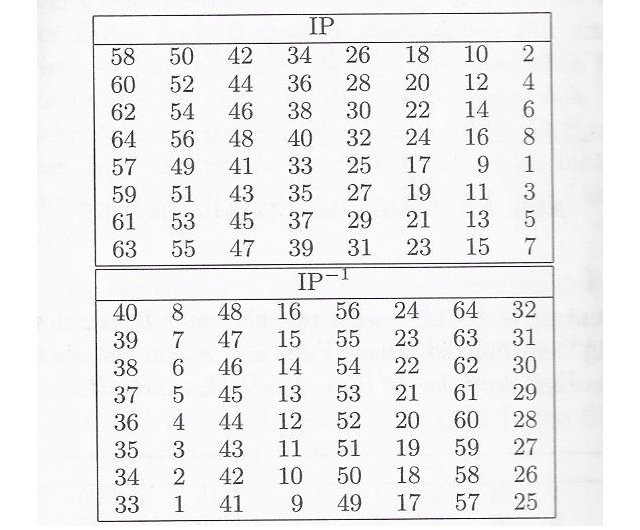
\includegraphics[width=.45\columnwidth]{PermutationsTabelle}} \quad
\caption[Eingangs-Permutations Tabelle]{Eingangs-Permuations Tabelle\footnotemark}
\label{fig:permutation}
\end{figure}
\footnotetext{\cite[Seite 105]{8}}
$\newline$
Jede Zahl beziffert genau die neue Position des Bits innerhalb des Permutatins-Blocks. So wird hier das erste Bit auf das 58te abgebildet, das zweite auf das 50te und so weiter. Nach dem selben Prizip wird dann die Expansion angewandt, allerdings ist dabei die Tabelle größer als der ursprüngliche Block. Das heißt hier werden manche Bits auf mehrere Stellen gesetzt.  
\subsection{Substitution}
Weiter wichtig sind zudem Substitutionen. Auf ihren Nutzen für die Sicherheit des Verfahrens wird später noch genauer eingegangen. Im Allgemeinen wird bei der Substitution ein Block an Bits durch einen anderen ersetzt. Dies geschieht wiederum durch Tabellen, wobei man hier beim DES auch von einer gleichzeitigen Kontraktion sprechen kann, da die Bitfolge verkürzt wird.
 \cite[Seite 107]{8} 

Expansion und Permutation sind lineare Abbildungen, wobei die Permutation eine Abbildung $\mathbb{Z}^{32}_2 \rightarrow \mathbb{Z}^{32}_2 $ und die Expansion eine Abbildung E: $ \mathbb{Z}^{32}_2 \rightarrow \mathbb{Z}^{48}_2 $sind.
Die Substitution ist eine nicht-lineare Abbildung. \cite[Seite 52]{2}
\section{Kryptologische Grundlagen}
	\subsection{Kryptosysteme - Simon Sternsdorf}
	Wir verwenden in dieser Arbeit die Definition eines Kryptosystems wie folgt: 
	Ein Kryptosystem ist ein Tupel(P, C, K, f, g) wobei P, C und K nicht leer sein dürfen. Hierbei ist: 
	\begin{itemize} 
		\item \textbf{P} die Klartextmenge, sprich der Text der verschlüsselt werden soll
		\item \textbf{C} die Geheimtextmenge, sprich der verschlüsselte Text
		\item \textbf{K} die Schlüsselmenge, also der Schlüssel der zum verschlüsseln der Klartextmenge zur Geheimtextmenge verwendet wurde
		\item \textbf{f} die Verschlüsselungsfunktion, eine Abbildung $f: P \, x\,  K \rightarrow C$ , die aus der Klartextmenge die Geheimtextmenge bildet
		\item \textbf{g} die Entschlüsselungsfunktion, eine Abbildung $g: C \, x \, K \rightarrow P$ , die aus der Geheimtextmenge die Klartextmenge bildet
	\end{itemize}

	Weiter muss gelten das $\forall k \in K : \exists k' \in K : g_{k'} \, o $ $ f_k = id_P $, was gleichbedeutent ist mit Injektivität und Surjektivität der Abbildung. Ohne diese Vorraussetzung wäre eine verschlüsselte Nachricht nicht mehr entschlüsselbar. Bei DES gilt $k' = k$. \cite[Seite 9]{2}
	\subsection{Perfekte Sicherheit - Simon Sternsdorf}
	\subsubsection{Konzept}
	Um zu verstehen wie sicher oder unsicher der DES-Algorithmus ist, braucht man das Konzept der perfekten Sicherheit. $\newline$ Hierbei gehen wir davon aus, dass der Angreifer über unendliche Rechenkapazitäten verfügt. Weiterhin haben wir ein Kryptosystem $ \pi = (P,C,K,f,g) $, das ein nach Kerckhoff's Prinzip sicheres Verschlüsselungsverfahren enthält, was heißt f und g sind allgemein bekannt. \cite{9}
	Wir haben nun Wahrscheinlichkeits-Verteilungen Ws auf P,C und K, zudem sind $\textit{P}, \textit{C}$ und $\textit{K}$ die Zufallsvariablen für die Ws-Verteilungen. Nun ziehen wir ein $p \in P$ mit $Ws[\textit{P} = p]$ und analog für C und K. Die Wahrscheinlichkeit für $\textit{P} = p$ und $\textit{C} = c$ sollen dabei $> 0$ sein. Nun ist unser Kryptosystem und damit unser Verschlüsselungsverfahren sicher wenn der folgende Satz gilt: 
	$\newline$
	
	\begin{theorem}
	[Chiffretext-Verteilung] 

	$$ Ws[ \textit{P} = p | \textit{C} = c] = Ws[\textit{P} = p] | \forall p \in P, c \in C $$  
	\end{theorem}
	\begin{proof} 
	Annahme: $\pi$ sei perfekt sicher. Dann gilt nach Satz von Bayes: 
	$$ \frac{Ws[ \textit{P} = p | \textit{C} = c] * Ws[\textit{P} = p]}{Ws[\textit{C} = c]} = Ws[ \textit{P} = p | \textit{C} = c] =  Ws[\textit{P} = p]$$

	Daraus folgt $$Ws[ \textit{P} = p | \textit{C} = c] = Ws[\textit{C} = c] $$
	Aus $Ws[ \textit{P} = p | \textit{C} = c] = Ws[\textit{C} = c]$ folgt mit dem Satz von Bayes:
	$$Ws[\textit{P} = p] = Ws[ \textit{P} = p | \textit{C} = c]$$
	Damit ist nachgewiesen, dass $\pi$ perfekt sicher ist.
	\end{proof}
	Der für diesen Satz nötige Satz lautet wie folgt: 
	$\newline$
	\begin{theorem}
	[Satz von Bayes]
	$\newline$
	Für zwei Ereignisse A und B, wobei $B \neq 0 $ : 
	$$ P_B (A) = \frac{P(A) * P_A (B)}{P(B)}$$ 
	Hierbei bezeichnet $P_B (A) $ die Wahrscheinlichkeit des Ereignisses A unter Vorraussetzung des Eintretens von Bedingung B.
	Equivalent für $P_A (B) $
	$P(A) $ ist die sogenante Anfangswahrscheinlichkeit für das Ereignis A. Sie meint, dass das Ereignis A unabhängig zu betrachten ist. \footnote{\url{http://matheguru.com/stochastik/36-satz-von-bayes.html} - 25.03.2016 15:50} 
	\end{theorem}
	\cite{10}
	Ein Angreifer der sowohl die entschlüsselte Nachricht wie auch die verschlüsselte besitzt hat mit diesem System keine Vorteile. \cite[Seite 5]{11}
	Man kann auch sagen p und c sind stochastisch unabhängig. 
	Mit dem Satz der Chiffren-Verteilung kann man folgendes nachweisen:
	\begin{theorem}
	[Ununterscheidbarkeit von Verschlüsselung]
	Ein Verschlüsselungsverfahren $\pi$ ist perfekt sicher wenn gilt: 
	$$p_0 , p_1 \in P, c \in C : Ws[ \textit{P} = p_0 | \textit{C} = c] =  Ws[ \textit{P} = p_1 | \textit{C} = c]$$
	\end{theorem}
	\begin{proof}
	Aus Satz 1 folgt für ein $\pi$ das perfekt sicher ist: 
	$$Ws[ \textit{P} = p_0 | \textit{C} = c] = Ws[ \textit{C} = c]$$
	$$ \exists c \in C : Ws[ \textit{C} = c] = Ws[ \textit{P} = p_1 | \textit{C} = c] $$
	Sei $ p' \in P$ frei wählbar. Dann gilt: 
	$$Ws[ \textit{C} = c] = \sum_{p \in P} Ws[ \textit{P} = p | \textit{C} = c] * Ws[ \textit{P} = p] $$
	$$ = Ws[ \textit{P} = p' | \textit{C} = c] * \sum_{p\in P} Ws[ \textit{P} = p]$$
	$$= Ws[ \textit{P} = p' | \textit{C} = c]$$
	Insgesamt folgt daraus die perfekte Sicherheit von $\pi$ \cite[Seite 6]{11}
	\end{proof}
	Man kann außerdem nachweisen, dass für das perfekte Verschlüsselungsverfahren gelten muss: 
	\begin{theorem}
	[Minimale Größe des Schlüsselraumes]
	Annahme: $\pi$ sei perfekt sicher. Dann gilt: $|K| \ge |P| $
	\end{theorem}
	\begin{proof}
	Beweis durch Widerspruch: 
	Annahme: $|K| < |P| $
	Für ein $c \in C$ definieren wir ein G(c) = {p | p = g(c,k) mit $k \in K$ }.
	Es muss $|G(c)| \le |K|$ gelten, da ein Schlüssel k genau einen Klartext p liefert.  
	Es gilt aber |K| < |P|. Daraus folgt das |G(c)| < |P|. Somit muss es ein $p \in P$ geben für das gilt: $Ws[\textit{P} = p | \textit{C} = c] = 0 < Ws[\textit{P} = p] $.
	Das würde bedeuten, dass $\pi$ nicht perfekt sicher sein kann, da die Ws als > 0 definiert wurden. \cite[Seite 8]{11}
	\end{proof}
	Mit dem Satz von Shannon können wir uns zudem noch die Verteilung der Schlüssel anschauen. 
	\begin{theorem} 
	[Shannon]
	Für ein Kryptosystem $\pi$ = (P,C,K,f,g) mit |P|=|C|=|K| gilt: $\pi$ ist perfekt sicher gdw : alle $k \in K$ werden durch f gleichverteilt gewählt mit einer Wahrscheinlichkeit von $ \frac{1}{|K|} $. Zudem gibt es für alle $p \in P, c \in C$ genau ein $k \in K $ sodass gilt: c = f(p,k).
	\end{theorem}
	Hier beweisen wir zunächst die Gegenrichtung($\Leftarrow$): 
	\begin{proof}
	Wir können ein $ c \in C$ genau zu einem $p \in P$ entschlüsseln mit einem $k \in K $, bedeutet g(c,k) = p. Dies geschieht mit $Ws[\frac{1}{|K|}] $ gleichverteilt. Wir folgern: 
	$$Ws[\textit{C} = c | \textit{P} = p] = \frac{1}{|K|}$$ für alle $p \in P$ 
	Hieraus folgt mit Satz 2: 
	$$Ws[\textit{C} = c | \textit{P} = p_0] = \frac{1}{|K|} = Ws[\textit{C} = c | \textit{P} = p_1]$$
	Die Hinrichtung ($\Rightarrow$) folgt somit:
	Widerspruchsbeweis:
	Wir nehmen an: $\exists (p,c)$ mit $c \ne f(p,k)$ für alle $k \in K $
	Deswegen gilt: $Ws[\textit{P} = p | \textit{C} = c] = 0 < Ws[\textit{P} = p]$. Dies steht im Widerspruch zu unserer Definition von einem perfekt sicherem System.
	
	Nehmen wir anders herum an: $\exists (p,c)$ mit $c = f(p,k)$ für mehrere $k \in K (\ge 2) $.
	Dann gilt: $\exists (p',c')$ mit $c' \ne f(p',k)$ für alle $k \in K $.
 
	Dies erzeugt einen Widerspruch wie oben. 
	Daraus folgern wir: Es gibt für jedes feste $p \in P, c \in C$ genau ein $k \in K$ für das gilt: f(p,k) = c. 
	Im weiteren ergibt sich für alle p, p' : 
	$Ws[\textit{K} = k_p] = Ws[\textit{C} = c | \textit{P} = p]$
	$ = Ws[\textit{C} = c | \textit{P} = p'] = Ws[\textit{K} = k_p']$
	$\rightarrow Ws[\textit{K} = k ] = \frac{1}{|K|}$ für alle $k \in K $ \cite[Seite 9]{11}
	\end{proof}
	$\newline$
	Intuitiv bedeutet perfekte Sicherheit also: $\newline$
	Der Schlüssel, der zur Verschlüsselung der Nachricht verwendet wird muss mindestens so lang sein wie die Nachricht selbst. Der Schlüssl muss zudem noch perfekt gleichverteilt von der Verschlüsselungsfunktion gewählt werden. Der Angreifer hat keinerlei Vorteile durch das Wissen um ein Klartext - verschlüsselter Text Paar. Das schließt auch sogenannte Meet-In-The-Middle Attacken aus, auf die später noch eingegangen wird. Mit all diesen nicht gerade leicht zu erfüllenden Bedingungen gibt es nicht viele Beispiele aus der Vergangenheit, von Verschlüsselungsverfahren die die Kriterien der perfekten Sicherheit erfüllten. 
	\subsubsection{Vernam'sches One-Time-Pad}
	Eines dieser wenigen Beispiel ist das Vernam'sche One-Time-Pad, eine 1918 von Gilbert Vernam entwickelte Verschlüsselungsmethode, die zum verschlüsseln des roten Telefons im Kalten Krieg zwischen dem US-Präsidenten und dem sowjetischen Generalsekretär genutzt wurde. Die Besonderheit ist, dass der Schlüssel genauso lang wie die zu verschlüsselnde Nachricht war. Zur Ver-und Entschlüsselung wurden Buchstaben nach einer Tabelle addiert. 
	
	\begin{figure}[h]
	\centering
	{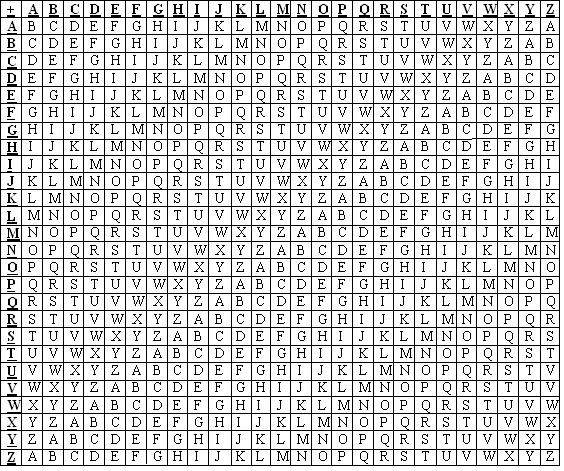
\includegraphics[width=.45\columnwidth]{OneTimePad}} \quad
	\caption[One-Time Pad Tabelle]{One-Time Pad Tabelle\footnotemark}
	\label{fig:Pad1}
	\end{figure}
	\footnotetext{\cite{12}}
	Addiert wurde mit einer zufälligen Buchstabenfolge die beiden Seiten bekannt war. \cite{12} Mathematisch wurde das One-Time-Pad definiert durch ein Kryptosystem $\pi = (P,C,K,f,g) $ wobei $ P=C=K=\{0,1\}^l $ für das gilt: 
	$$ \exists k \in K, \exists p \in P : c \in C = f(p,k) = p \oplus k$$
	$$ \exists k \in K, \exists c \in C : p \in P = g(c,k) = c \oplus k$$h
	Annahme: Das One-Time-Pad ist ein perfekt sicheres Verfahren. 
	\begin{proof}
	Da $\textit{C} = \textit{P} \oplus \textit{K}$ gilt: 
	$\forall p_0 , p_1 \in P und c \in C : Ws[\textit{C} = c | \textit{P} = p_0 ] = Ws[\textit{P} \oplus \textit{K} = p_0 ] = Ws [\textit{K} = p_0 \oplus c] $
	$ = \frac{1}{2^l} = Ws[\textit{C} = c | \textit{P} = p_1 ]$
	\end{proof}
	Dies entspicht dem Satz über Ununterscheidbarkeit von Verschlüsselung.
	Somit ist das One-Time-Pad perfekt sicher. \cite[Seite 7]{11} $\newline$
	Das Beispiel zeigt gut, wie wenig praktikabel eine Verschlüsselung mit perfekter Verschlüsselung im Alltag ist. Ein so langer Schlüssel macht nicht nur das Ver- und Entschlüsseln langsam, sondern fördert auch das Auftreten von Fehlern. Wenn beim One-Time-Pad die zufälligen Buchstabenfolgen nicht übereinstimmten oder etwa falsch gelesen wurden, konnten beide Seiten nicht mehr kommunizieren und es mussten neue Folgen ausgetauscht werden, was wiederum anfällig für Fehler und Angriffe von 3ten Parteien war. Somit kann das Ziel bei der Konstruktion eines Verschlüsselungsalgorithmus nie sein, ihn perfekt sicher zu machen, sondern nur sicher genug.
	$\newline$
	In der Realität haben die Angreifer auf eine Verschlüsselung nie unbegrenzte Resourcen zur Verfügung. Somit ist ein Schlüssel, der sehr viel kürzer als die Länge des Klartextes ist, oftmals ausreichend. 
	Auch ist die Wahl eines Algorithmus, der die Schlüssel absolut gleichverteilt wählt, sehr schwierig und nur bei einem riesigem Schlüsselraum realistsisch. Ein solches Verschlüsselungsverfahren zu bauen und zu verwalten ist nicht praktisch. 

	\subsection{Diffusion und Konfusion - Alexej Rotar}
	
	Ein Verschlüsselungsverfahren, das die Redundanz, bzw. Struktur einer Nachricht beim Verschlüsseln beibehält, kann gut analysiert werden. Denn es kann dann der Geheimtext nach solchen Strukturen untersucht werden und so können gewisse Schlüssel mit höherer Wahrscheinlichkeit ausgewählt, bzw. ausgeschlossen werden.  \cite[52]{4} Von Shannon wurden zwei allgemeine Methoden entwickelt, die solche Analysen erschweren.

	\subsubsection{Diffusion}
	Bei der Diffusion geht es darum, die Struktur einer Nachricht zu zerstören, sodass die Redundanz auf größere Strukturen verteilt wird. So tritt immer noch Redundanz auf, jedoch nur bei den größeren Strukturen. Die Wahrscheinlichkeiten für einzelne Strukturen sinken dadurch. Daher müssen wesentlich mehr Nachrichten abgefangen werden, um statistische Analysen betreiben zu können. \cite[53-54]{4} Konkret bedeutet das, dass sich jedes Zeichen eines Klartexts auf möglichst viele Zeichen des Geheimtexts auswirken muss. Die Veränderung eines einzelnen Zeichens führt im Idealfall zur Veränderung eines jeden Zeichens im Geheimtext mit Wahrscheinlichkeit $\frac{1}{2}$. \cite[45]{2} 

	\subsubsection{Konfusion}
	Konfusion veschleiert den Zusammenhang zwischen dem Geheimtext und dem Schlüssel. So wird ein statistischer Angriff ebenfalls erschwert. Denn so muss unter Umständen ein komplexes Gleichungssystem gelöst werden, um einen Schlüssel zu ermitteln. Damit ein Verfahren konfus ist, sollte sich möglichst jeder Teil des Schlüssels auf die Geheimnachricht auswirken. \cite[54-55]{4}
	
	\subsubsection{Konstruktion einer sicheren Chiffre}
	Eine Möglichkeit, ein Verfahren zu konstruieren, welches diffus und konfus ist, ist es ein Verfahren zu iterieren, bei dem sich Substitutionen mit Permutationen abwechseln. Damit man dasselbe Verfahren mehrfach anwenden kann, ist es notwendig, dass es sich um eine \emph{endomorphe} Chiffre handelt. Das heißt, es müssen Bild- und Urbildmenge diesselbe sein. \cite[111]{3}

	
\section{Blockchiffren - Alexej Rotar}
	\subsection{Allgemein}
	Bei Verfahren wie beispielsweise der Caesar-Chiffre wird jedes Zeichen einzeln verschlüsselt. Bei manchen Verfahren werden dagegen ganze Blöcke verschlüsselt. Dann spricht man von \emph{Blockchiffren}. Dabei wird eine Nachricht $P$ in mehrere Blöcke der Länge $l$ aufgeteilt. Sollte $l$ kein Teiler der Länge von $P$ sein, wird der letzte Block mit weiteren Zeichen entsprechend aufgefüllt. Diese Zeichen nennt man auch \emph{Padding}. \\
	Nun wird jeder Block mit demselben Schlüssel $k$ verschlüsselt. Man erhält dieselbe Anzahl verschlüsselter Blöcke. Zusammen bilden die Blöcke die verschlüsselte Nachricht $C$. \cite[33]{2}

	\subsection{Feistel-Chiffren}
	Eine Spezialisierung der Blockchiffren sind die sogenannten \emph{Feistel-Chiffren}. Im Folgenden soll zunächst auf ihre Struktur und anschließend auf ihre Entschlüsselung eingegangen werden.

	\subsubsection{Struktur}
	Eine Feistel-Chiffre ist eine endomorphe Blockchiffre mit einer festgelegten Rundenanzahl. Sie wird festgelegt durch eine sogenannte \emph{innere Blockchiffre} $B$, eine Rundenanzahl $N \in \mathbb{N}$, eine Schlüsselmenge $\tilde{K}$ und eine Schlüsselauswahlfunktion $\phi$. Dabei ist $B$ definiert durch
	$$ B := (\mathbb{Z}^n_2, \mathbb{Z}^n_2, K, f) \footnote{Hier wurde die Funktion $g$ bewusst weggelassen, da für die interne Blockchiffre keine Entschlüsselungsfunktion notwendig ist.} $$

	Dann ist die Feistel-Chiffre definiert durch 
	$$ F := (\mathbb{Z}^{2n}_2, \mathbb{Z}^{2n}_2, \tilde{K}, \tilde{f}, \tilde{g}) $$

	Nun wird zunächst eine Klartextnachricht $P \in \mathbb{Z}_{2}^{2n}$ in eine linke und eine rechte Hälfte $L_0,\ R_0 \in \mathbb{Z}_{2}^n$ geteilt. Das heißt $P = (L_0, R_0)$. Anschließend wird rekursiv berechnet

	\begin{align} 
		L_i &:= R_{i-1}\label{eq4.1} \\
		R_i &:= L_{i-1} \oplus f(R_{i-1}, k_i) \label{eq4.2}
	\end{align}
	
	für $i \in \{1, \dots, N \}$. Dabei ist $\oplus$ eine bitweise XOR-Verknüpfung. Der Vektor $(k_1, \dots, k_N)$ wird durch die Funktion $\phi : \tilde{K} \rightarrow K^n$ vorgegeben. Die $k_i$ werden als \emph{Rundenschlüssel} bezeichnet. Die Funktion

	$$ \tilde{f}: \mathbb{Z}_{2}^{2n} \times \tilde{K} 
	\rightarrow \mathbb{Z}^{2n}_2, (P,k) \mapsto (R_N, L_N) $$
	
	beschreibt schließlich eine Verschlüsselung mit einer Feistel-chiffre. \cite[51]{2} Hier ist insbesondere zu beachten, dass nun $R_N$ links, während $L_N$ rechts steht. Der Grund hierfür wird im nächsten Abschnitt ersichtlich. Der Ablauf kann folgendermaßen veranschaulicht werden: 

	\begin{figure}[ht]
	\centering
	\input{../grafiken/feistel/feistel_input.tex}
	\label{fig:feistel}
	\caption[Ablauf einer Feistel-Chiffre] {Ablauf einer Feistel-Chiffre \cite[128]{3}}
	
	\end{figure}


	\subsubsection{Entschlüsselung}
	Es sei die Chiffre $C := (R_N, L_N)$ unser Ausgangspunkt. Nun soll hieraus wieder die ursprüngliche Nachricht $P := (L_0, R_0)$ ermittelt werden. Wir wollen zeigen, dass sich die Nachricht mittels Anwendung desselben Algorithmus bestimmen lässt. Dazu zeigen wir zunächst ein Lemma.
	
	\begin{lemma}
		Der Algorithmus lässt sich umkehren unabhängig davon, wie die Funktion $f$ definiert ist.
	\label{l1}
	\end{lemma}

	\begin{proof}
	Durch Umformung von \ref{eq4.1}, bzw. \ref{eq4.2} nach $R_{i-1}$, bzw. $L_{i-1}$ erhält man

	\begin{align}
		R_{i-1} &= L_i \label{eq4.3} \\
		\begin{split}
		L_{i-1} &= R_i \oplus f(R_{i-1}, k_i) \\ 
				&= R_i \oplus f(L_i, k_i) \label{eq4.4}
		\end{split}
	\end{align}
		
	\end{proof}

	Es kann also aus einem Nachfolger der entsprechende Vorgänger ermittelt werden. \cite[51]{2}

	\begin{theorem}
	Die Umkehrung des Algorithmus ist gerade derselbe Algorithmus, wobei die Rundenschlüssel in umgekehrter Reihenfolge verwendet werden. 
	\label{t1}
	\end{theorem}

	\begin{proof}
	Es wurde bereits festgestellt, dass in der resultierenden Chiffre die linke und rechte Hälfte aus dem letzten Schritt vertauscht sind. Wir definieren daher die beiden Hälften neu:

	$$ L'_0 := R_N $$
	$$ R'_0 := L_N $$

	Wir definieren weiterhin $j := N-i$, also folgt $i = N-j$. Außerdem folgt $N-(j+1) = N-j-1 = i-1$. Da nach jeder Runde die linke und rechte Hälfte vertauscht werden, ergibt sich mit dieser Definition
	
	\begin{align*}
		R'_j &:= L_{N-j} = L_i \\
		L'_j &:= R_i
	\end{align*}

	und außerdem

	$$ R'_{j+1} = L_{i-1} $$
	$$ L'_{j+1} = R_{i-1} $$ \\
	
	Durch Einsetzen in \ref{eq4.3}, bzw. \ref{eq4.4} ergibt sich

	\begin{align*}
		L'_{j+1} &= R'_j \\
		R'_{j+1} &= L'_j \oplus f(R'_j, k_i)
	\end{align*}

	Nach einem Indexshift und Umbenennung der Rundenschlüssel zu $k'_j := k_{N-(j-1)} = k_{N-j+1} = k_{i+1}$ ergibt sich gerade die ursprüngliche Rekursionsformel
	
	\begin{align*}
		L'_j &= R'_{j-1} \\
		R'_j &= L'_{j-1} \oplus f(R'_{j-1}, k'_j)
	\end{align*}
\end{proof}

	Die Umbenennung der Schlüssel bedeutet dabei, dass die Schlüssel in umgekehrter Reihenfolge angewandt werden. Der Versatz um eins ist notwendig, da wir bei den Schlüsseln bei $1$ zu zählen beginnen.

\section{DES - Alexej Rotar}
  
	\subsection{Allgemein}
	Der DES-Algorithmus ist eine Feistel-Chiffre mit interner Blockchiffre 
	
	$$ B = (\mathbb{Z}^{32}_2 , \mathbb{Z}^{32}_2 , \mathbb{Z}^{48}_2, f) $$
	
	und $ N = 16 $ Runden.\cite[51-52]{2} Nach der Definition der Feistel-Chiffren folgt daraus, dass 64-Bit-Blöcke verschlüsselt werden und die Rundenschlüssel 48-Bit breit sind. Auf die Funktion $f$ wird anschließend genauer eingegangen.

	Eine Besonderheit des DES sind die Eingangs- und Ausgangspermutation \emph{IP}, bzw. \emph{FP} (initial, bzw. final permutation). Dabei ist die Ausgangspermutation definiert als

	$$ FP := IP^{-1} $$
	
	Sie werden einmalig vor, bzw. nach dem Algorithmus ausgeführt. Da die Permutationen bekannt sind und nur am Anfang, bzw. am Ende ausgeführt werden, tragen sie nicht direkt zur Sicherheit des Verfahrens bei. Ein möglicher Grund für deren Verwendung könnte deren einfache hardwaretechnische Implementierung sein. Denn um eine Permutation in Hardware zu realisieren, kann man einfach entsprechend Ein- und Ausgänge direkt verdrahten. Softwaretechnische Implementierungen sind dagegen wesentlich aufwändiger und auch weniger effizient. Dadurch verlieren auch mögliche softwarebasierte Angriffe an Effizienz. Bei den heutigen Prozessoren spielt das allerdings keine Rolle mehr. 	
	Aufgrund der Definition von $FP$ als Umkehrung von $IP$ lässt sich auch der DES-Algorithmus entschlüsseln, indem derselbe Algorithmus erneut angewandt wird, so wie es bei den Feistel-Chiffren üblich ist.
	
	\subsection{Die Rundenfunktion}
	Die Funktion $f$ ist der Kern des DES-Verfahrens. Sie ist definiert als
	
	$$ f(R,k) \mapsto \pi (S(E(R) \oplus k)) $$
	
	wobei $k$ der Rundenschlüssel ist und $R \in \mathbb{Z}^{32}_2$ die aktuell rechte Hälfte. \cite[52]{2} Die einzelnen Funktionen sind folgendermaßen definiert:

	\subsubsection{Die Expansion}
	Die Abbildung $ E: \mathbb{Z}^{32}_2 \rightarrow \mathbb{Z}^{48}_2 $ ist 
definiert durch die Tabelle \ref{tab:exp}.
	
	\begin{table}[ht]
	\input{../grafiken/expansion/expansion_input.tex}
	\caption{Expansionsabbildung \cite[52]{2}}
	\label{tab:exp}
	\end{table}
	
	Es fällt auf, dass stets das letzte und das erste Bit eines 4-Bit-Blocks verdoppelt werden. Das heißt es werden 16 Bits ergänzt, sodass der resultierende Block 48 Bit breit ist. \cite[52]{2} \\
	Da sie sich als Matrixmultiplikation darstellen lässt, handelt es sich bei der Expansion um eine lineare Abbildung. Sie erhält außerdem weitgehend die Struktur des Blocks und kann somit nicht der Diffusion dienen. Allerdings ist sie notwendig, um die Nachricht auf die Größe eines Rundenschlüssel zu bringen, der anschließend damit addiert wird.
	
	\subsubsection{Die Substitution}
	Die Abbildung $ S: \mathbb{Z}^{48}_2 \rightarrow \mathbb{Z}^{32}_2 $ bildet den nun entstandenen 48-Bit-Block auf die urpsprüngliche Größe von 32 Bit ab, damit mit diesem anschließend, wie von Feistel-Chiffren gewohnt, weitergearbeitet werden kann. Dabei werden insgesamt acht 6-Bit-Blöcke durch wiederum acht 4-Bit-Blöcke ersetzt. Dazu werden die sogenannten \emph{S-Boxen} verwendet. Es dient stets der erste Block als Eingabe für $S_1$, der zweite für $S_2$ und so weiter. Die folgende Tabelle zeigt exemplarisch eine solche S-Box.
	
	
	\begin{1}[ht]
	\input{../grafiken/sbox/sbox_input.tex}
	\caption{S-Box $S_5$ \cite[52]{2}}
	\label{tab:sbox}
	\end{table}
	
	Aus der Abbildung erkennt man, dass eine S-Box vier Zeilen enthält. Jede dieser Zeilen ist eine Substitution. Welche Substitution verwendet wird, entscheiden das Bit 1 und 6 des Eingabeblocks. Das heißt, es wird für einen Block $ (b_1,b_2,b_3,b_4,b_5,b_6) $ die Substitution $ b_1b_6 $ verwendet. Die übrigen Stellen, die Zahlen von 0 bis 15 darstellen können, bilden die zu ersetzende Zahl, entscheiden also, welche Spalte einer S-Box verwendet wird. \cite[138]{3} An einem einfachen Beispiel sieht man schnell, dass die Substitution keine lineare Abbildung ist.
	
	\subsubsection{Die Permutation}
	Die Abbildung $ \pi: \mathbb{Z}^{32}_2 \rightarrow \mathbb{Z}^{32}_2 $ permutiert schließlich das Ergebnis der Substitution gemäß Tabelle \ref{tab:perm}.

	\begin{table}[ht]
	\input{../grafiken/permutation/permutation_input.tex}
	\caption{Permutationsabbildung \cite[139]{3}}
	\label{tab:perm}
	\end{table}

	An der Tabelle sieht man, dass der Block durch die Permutation zerstreut wird. Somit wirkt sich jeder Teil der Nachricht an vielen Stellen der Geheimnachricht aus, wodurch das Verfahren diffus wird. Ähnlich wie die Expansion, ist auch die Permutation eine lineare Abbildung.
	
	\subsection{Die Schlüsselauswahlfunktion}
	Wie aus dem Abschnitt über Feistel-Chiffren bekannt, ist eine Schlüsselauswahlfunktion $\phi$ notwendig, die aus der Schlüsselmenge $\mathbb{Z}^{64}_2$ die 16 Rundenschlüssel bildet. Beim DES werden nur 56-Bit des Schlüssels berücksichtigt, da die übrigen 8 Paritätsbits sind. \cite[133]{3} Daher werden zunächst die 56 relevanten Bits ausgewählt und auf zwei 28-Bit Register, $C$ und $D$, verteilt. Dazu wird die Permutation PC-1 verwendet. Anschließend werden die 16 Rundenschlüssel gebildet, indem zunächst beide Register nach folgendem Schema rotiert werden:

	\input{../grafiken/keyrotation/keyrotation_input.tex}

	Das heißt, es wird jeweils vor der entsprechenden Runde rotiert. Nach jeder Rotation wird mittels der Permutation PC-2 der entsprechende Rundenschlüssel gebildet.

	Ähnlich wie die Anfangs- und Endpermutationen wirkt sich PC-1 nicht auf die Sicherheit des Verfahrens aus, da sie nur einmalig zu Beginn angewandt wird. Sie dient im Grunde lediglich der Auswahl der für den Schlüssel relevanten Bits. \cite[141]{3} Die Rotation und PC-2, dagegen, sorgen dafür, dass die Bits des Schlüssels sich an möglichst vielen Stellen auf die Chiffre auswirken und damit für eine hohe Konfusion. Denn es fällt auf, dass die Summe der 1-Bit-Rotationen 28 ergibt, also gerade die Größe eines Registers. Damit wird gewährleistet, dass die Schlüsselbits sich gleichmäßig über die gesamte Chiffre verteilen. Der letzte Schlüssel $k_{16}$ wird aus den ursprünglichen Registern $C$ und $D$ gebildet.
	
	\subsection{Sicherheit}
	Bei der Betrachtung der einzelnen Teilfunktionen des DES wurden bereits deren Auswirkungen auf die Sicherheit angesprochen. Im Großen und Ganzen sieht man nun, dass das DES sowohl einen hohen Grad an Diffusion wie an Konfusion aufweist. Es fällt außerdem auf, dass hier genau die von Shannon vorgeschlagene Vorgehensweise verwendet wird. In jeder Runde findet eine Permutation und eine Substitution statt und das Verfahren wird iteriert. 

	Als einzige nicht-lineare Funktion sorgt die Substitution auch für die nicht-Linearität des gesamten Verfahrens und ist damit ein entscheidender Faktor für dessen Sicherheit. Denn lineare Abbildungen lassen sich sehr gut analysieren. \cite[21]{2} Damit ist die richtige Wahl der S-Boxen von großer Bedeutung. Es hat sich herausgestellt, dass bei kleinen Änderungen einer der S-Boxen das Verfahren bereits wesentlich unsicherer wird. Wie genau die richtigen S-Boxen ermittelt wurden ist allerdings nicht bekannt. \cite[52]{2}

\section{Kryptoanalyse - Alexej Rotar}
	Bei der Kryptoanalyse geht es darum, aus abgefangenen Nachrichten Informationen über die Klartextnachricht oder den Schlüssel abzuleiten. Man unterscheidet dabei unterschiedliche Arten. Für uns sind die relevanten \emph{Known-Plaintext-Angriff} und \emph{Chosen-Plaintext-Angriff}. Bei ersterem kennt der Angreifer zu einem Geheimtext auch den Klartext, während er bei letzterem zu jedem beliebigen Klartext den Geheimtext erlangen kann. \cite[24]{1} \\
	Es wurden für einen Angriff gegen den DES zwei Methoden vorgestellt. Wir beschränken uns auf die \emph{Differentielle Kryptoanalyse}.

	\subsection{Das Ziel}
	Das Ziel der differentiellen Kryptoanalyse ist es, einen Teilschlüssel zu bestimmen. Hat man beispielsweise einen gesamten 48-Bit-Rundenschlüssel gefunden, so bleiben nur noch 8 relevante Bits übrig, die leicht mittels Brute-Force ermittelt werden können. \cite[153]{3} Im Folgenden gelten die Bezeichnungen

	\begin{itemize}
	\item $x,x'$ : Eingaben für eine Rundenfunktion
	\item $y,y'$ : Ausgaben einer Rundenfunktion
	\item $\Delta x, \Delta y$ : Ein-,Ausgabedifferenz der Rundenfunktion
	\item $e, a$ : Ein-, Ausgabe einer S-Box
	\item $\Delta e, \Delta a$ : Ein-, Ausgabedifferenz einer S-Box
	\end{itemize}

	Aufgrund der Definition einer Rundenfunktion gilt der Zusammenhang
	
	\begin{equation}
		k^{(1)} = e^{(1)} \oplus E^{(1)}(x)  
	\label{eq:key}
	\end{equation}

	Wobei damit jeweils die ersten 6 Bits des Schlüssels, der Eingabe, bzw. der Expansion gemeint sind. Man kann also leicht einen Teilschlüssel ermitteln, wenn $e$ bekannt ist. Dieses kann allerdings nicht ohne Weiteres ermittelt werden, wenn der Schlüssel unbekannt ist. Daher betrachtet man bei der Differentiellen Kryptoanalyse Differenzen anstatt einzelner Werte.

	\subsection{Differenzenverteilung}
	Es seien nun $x,x',y,y'$ gegeben und damit auch $\Delta x = x \oplus x'$, bzw. $\Delta y = y \oplus y'$. Aus $\Delta y$ lässt sich leicht $\Delta a$ bestimmen durch

	$$ \Delta a = (P^{-1}(y)) \oplus (P^{-1}(y') = P^{-1} (\Delta y) $$

	Wobei die letzte Gleichheit gilt, weil $P$ eine lineare Abbildung ist. \cite[160]{3} Für die Eingabedifferenz gilt

	$$ \Delta e = (E(x) \oplus k) \oplus (E(x') \oplus k) = E(\Delta x) $$

	Es lässt sich also auch die Eingabedifferenz ohne Kenntnis des Schlüssels bestimmen. \cite[139]{3} Nun stellt sich die Frage, inwiefern Ein- und Ausgabedifferenzen der S-Boxen zusammenhängen. Da die S-Boxen nicht-lineare Abbildungen sind, lässt sich kein Zusammenhang wie bei den Abbildungen $E$ und $P$ herstellen. Jedoch kann man bei bekanntem $\Delta x$ 64 unterschiedliche Paare $x,x'$ finden, die diese Differenz bilden. Nun kann zu jedem dieser Paare die Ausgabedifferenz

	$$ \Delta a = S(x) \oplus S(x') $$

	betrachtet und mit der gegebenen verglichen werden. Im Allgemeinen werden mehrere Eingabepaare dieselbe Ausgabedifferenz erzeugen, da $S$ keine Injektive Abbildung ist. \cite[155-156]{3} Jedes dieser Paare ist potentiell richtig und bildet mit Formel \ref{eq:key} einen Schlüssel. Die Menge dieser potentiellen Schlüssel wird Kandidatenmenge $\mathcal{K}_{x,x'}$ genannt. Wiederholt man diesen Vorgang mit unterschiedlichen Eingabedifferenzen, ergeben sich unterschiedliche Kandidatenmengen, von denen aber jede den richtigen Schlüssel enthält. Die Schnittmenge einiger solcher Mengen ergibt schließlich den richtigen Schlüssel. \cite[160]{3} \\
	Die unterschiedlichen Ein- und Ausgabedifferenzen mit entsprechenden Eingabepaaren können in 64 Tabellen mit 64 Zeilen und 16 Spalten pro S-Box festgehalten werden. Die Anzahl der Eingabepaare, die eine bestimmte Ausgabedifferenz erzeugen, kann ebenfalls in einer Tabelle festgehalten werden, die \emph{Differenzenverteilung} genannt wird. \cite[156]{3}

	\subsection{Bestimmung der Differenzen}
	Man kann mit unterschiedlichen Methoden die Ein- und Ausgabedifferenzen des DES mit bis zu fünf Runden bestimmen. Ab sechs Runden ist das nicht mehr mit Sicherheit möglich. Stattdessen kann man nur noch mit gewissen Wahrscheinlichkeiten die Differenzen vorhersagen. Zunächst sollen nun einige Hilfsmittel definiert werden, um anschließend gewisse Aussagen über die Differenzen und Schlüssel treffen zu können.

	\begin{definition}
	Es sei $P(S_j, \Delta e \rightarrow \Delta a)$ die Wahrscheinlichkeit, dass die Eingabedifferenz $\Delta e$ die Ausgabedifferenz $\Delta a$ erzeugt. Es gilt

	$$ P(S_j, \Delta e \rightarrow \Delta a) :=
		\frac{| \{(e,e') | e \oplus e' = \Delta e 
		\wedge S_j(e) \oplus S_j(e') = \Delta a\} |}{64} $$

	\end{definition}

	\begin{definition}
	Es sei weiterhin $P(f, \Delta x, \rightarrow \Delta y)$ die Wahrscheinlichkeit, dass $\Delta x$ mit $F$ die Differenz $\Delta y$ erzeugt. Es gilt

	$$ P(F, \Delta x \rightarrow \Delta y) := 
		\frac{| \{ (x,x',k) | x \oplus x' = \Delta x 
		\wedge F(k,x) \oplus F(k,x') = \Delta y \} |}{2^{32} \cdot 2^{48}} 
	\cite[164-165]{3} $$

	\end{definition}


	\begin{theorem}
	Zwischen den eben definierten Wahrscheinlichkeiten gilt folgender Zusammenhang:

	$$ P(F, \Delta x \rightarrow \Delta y) =
		\prod_{j=1}^8{P(S_j, \Delta e^{(j)} \rightarrow \Delta a^{(j)})} $$

	\end{theorem}

	Nun wollen wir unsere Differenzen über mehrere Runden hinweg nachverfolgen. Dafür brauchen wir die sogenannte \emph{DES-Charakteristik}. 
	
	\begin{definition}
	Die DES-Charakteristik ist definiert als $\Gamma := (\Delta m, \lambda, \Delta c)$, wobei

	\begin{itemize}
	\item $\Delta m$ die Eingabedifferenz des DES,
	\item $\Delta c$ die Ausgabedifferenz des DES und
	\item $\lambda := (\lambda_1, \dots, \lambda_n)$ eine Liste mit Differenzen der einzelnen Runden ist. Dabei ist $\lambda_i = (\Delta x_i, \Delta y_i)$.
	\end{itemize}
	\end{definition}

	Es erzeugt $\Delta m$ die Ausgabe $\Delta c$ gemäß $\Gamma$ mit der Wahrscheinlichkeit

	$$ p^{\Gamma} := \prod_{i=1}^n{P(F, \Delta x_i \rightarrow \Delta y_i)} \cite[166-167]{3} $$
	Wir wollen nun Nachrichten unterscheiden, welche die richtige Ausgabedifferenz erzeugen, von solchen, die falsche erzeugen.

	\begin{definition}
	Es sei ein Schlüssel $K$ und eine Charakteristik $\Gamma$ gegeben. Das Klartextpaar $M, M'$ heißt $(\Gamma, K$)-treu, falls die folgenden Bedingungen gelten:

	\begin{itemize}
	\item $\lambda_i = (\Delta x_i, \Delta y_i)$ für alle $i$. Dabei sind $\Delta x_i$, bzw. $\Delta y_i$ die Ein- und Ausgabedifferenzen der Rundenfunktionen bei der Verschlüsselung von $M$ und $M'$.
	\item $C \oplus C' = \Delta c$.
	\end{itemize}
	\end{definition}

	Nun ist ein Paar $M,M'$ mit der Wahrscheinlichkeit $p^{\Gamma}$ $(\Gamma, k)$-treu. Es kann jetzt wie zuvor beschrieben eine Kanditatenmenge für den Schlüssel aus einem Klartextpaar und einer Geheimtextdifferenz abgeleitet werden. Sollte das Klartextpaar $(\Gamma, K)$-treu sein, enthält die Kanditatenmenge auf jeden Fall den richtigen Schlüssel. Andernfalls ist das nicht zwangsläufig der Fall. Daraus folgt also, dass mit Wahrscheinlichkeit $p^{\Gamma}$ der richtige Teilschlüssel in einer Kanditatenmenge enthalten ist. Es hat sich gezeigt, dass der richtige Teilschlüssel am häufigsten in den Mengen vorkommt. Daher kann dieser gefunden werden, wenn eine genügend hohe Anzahl Klartextpaare überprüft wird. \cite[172-174]{3}

\section{Schluss - Simon Sternsdorf}
\subsection{Kritik an DES} 
Schon recht früh nach Einführung des DES-Algorithmus als Standard-Verschlüsselung in vielen Bereichen des Öffenlichen Lebens kam Kritk auf. So wurde bereits früh, im Jahr 1975, vor der Möglichkeit eines Brute-Force Angriffs gewarnt, der aufgrund der recht kurzen Schlüssellänge gut möglich wäre. Im speziellen Martin Hellman und Whitfield Diffie, die Erfinder des Konzepts der Public-Key Verschlüsselung, warnten vor möglichen Angriffen von Regierungsorganisationen, im speziellen Geheimdienste. Diese hätten Zugriff auf die für damalige Verhältnisse recht hohe Rechenleistung. \cite{6}
\subsection{Brute-Force}
Ein Brute-Force-Angriff ist die einfachste und gewaltsamste Art eine Verschlüsselung zu knacken. Dabei wird von einem Computer systematisch jede Kombination aus Zahlen, Buchstaben und Sonderzeichen bis zu einer zuvor festgelegten Länge durchprobiert. Je kürzer dabei die Länge des verwendeten Schlüssels ist desto schneller ist das Verfahren. Zudem hängt es von der verwendeten Rechenpower des Angreifers ab. Ein höherer Einsatz von Rechenleistung erhöht die Geschwindigkeit der Suche. \cite{13} $\newline$
Moderne Verschlüsselungen setzen deswegen heutzutage auf Schlüssel, die sehr viel länger sind als die 56 Bit des DES-Algorithmus. Der weit verbreitete Verschlüsselungsalgorithmus AES setzt auf Schlüssellängen bis zu 256 Bit. \cite{14}
\subsection{Der DES-Cracker} 
Im Jahr 1998 gelang es schließlich der Electronic Frontier Foundation, eine Organisation die sich für digitale Grundrechte und Privatssphäre einsetzt, mithilfe einer selbst gebauten "'Crackers"' den DES-Algorithmus mittels Brute-Force zu knacken. Die Maschine kostete nur 250.000 Dollar und benötigte nur 3 Tage um diese Aufgabe zu bewerkstelligen. Die EFF wollte damit der Öffentlichkeit aufzeigen, wie leicht der immer noch in weiten Teilen der Industrie eingesetzte Verschlüsselungsalgorithmus zu knacken war.
\begin{figure}[tb]
\centering
\subfloat[Der verwendete Cracker-Chip.]{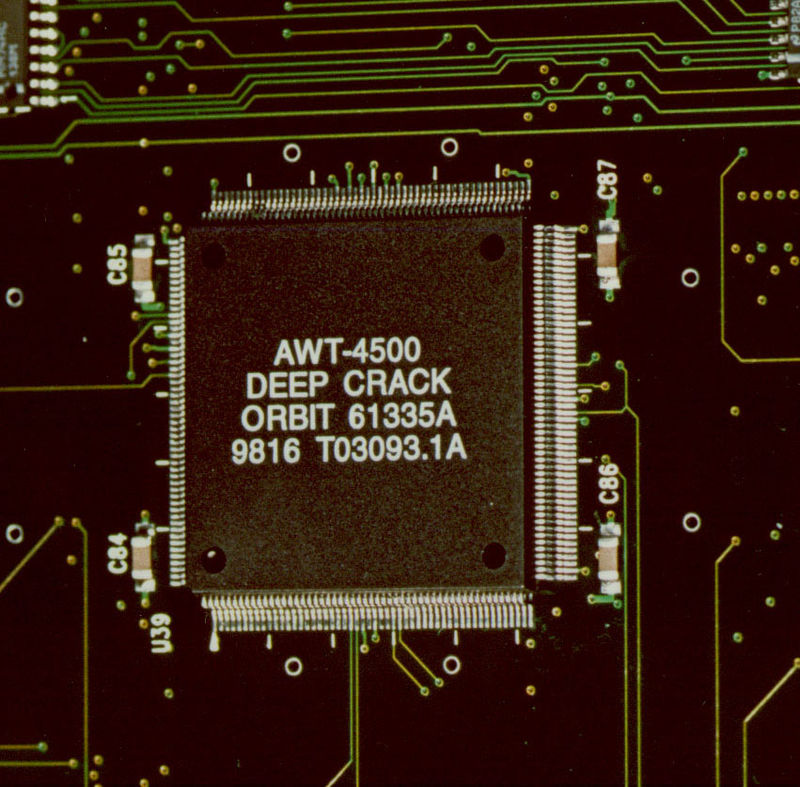
\includegraphics[width=.45\columnwidth]{Chip300}} \quad
\subfloat[Ein Chip-Board]{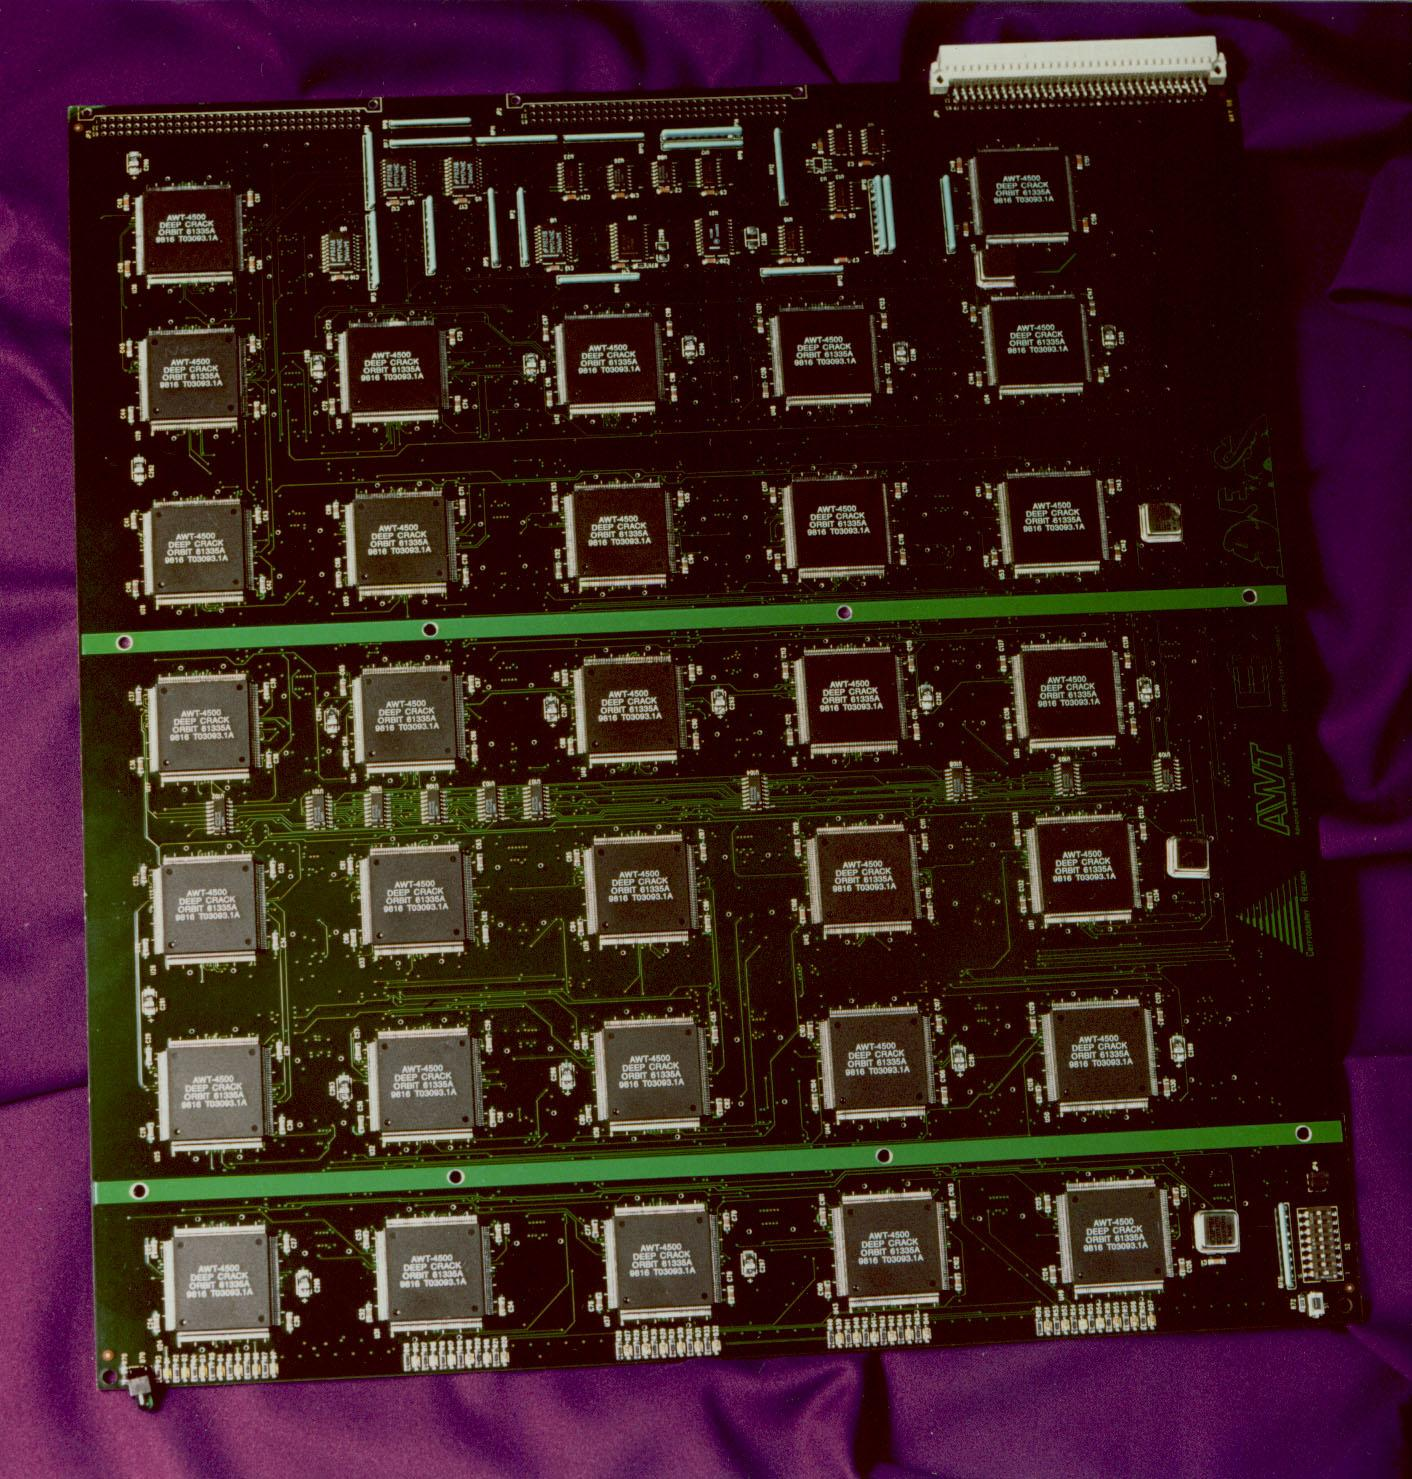
\includegraphics[width=.45\columnwidth]{board300}\label{fig:Chip}} \\
\caption[DES-Cracker.]{DES-Cracker Chip \footnotemark}
\label{fig:ChipBoard}
\end{figure}
\footnotetext{\cite{15}}
1999 gelang es mit dem DES-Cracker und einem weltweitem Computernetzwerk namens Distributed.Net eine DES-verschlüsselte Nachricht in nur 22 Stunden zu knacken. Die Computer schafften es zusammen auf eine Geschwindigkeit von 245 Millarden Schlüsseltests pro Sekunde. Das ganze geschah im Rahmen eines Wettbewerbs, um die von der US-Regierung immer noch bestehende Behauptung zu widerlegen, dass es Jahre brauchen würde und Rechenleistung im Wert von mehreren Millionen Dollar um eine DES-Nachricht mittels Brute-Force zu entschlüsseln. \cite{15}
\subsection{Entwickelte Alternativen} 
Die EFF schlug schon 1994 dem X9 Kommittee, das für die Empfehlung von neuen Verschlüsselungsalgorithmen verantwortlich war als Alternative triple-DES oder kurz 3DES vor. Damit stellten sie sich klar gegen die NSA und deren Vorschlag eines speziellen Verschlüsselungschips namens Clipper, der einen eingebauten "'Backdoor"' enthielt, um so der NSA Zugriff auf verschlüsselte Kommunikation zu geben. Ein Backdoor ist eine Hintertür in einem eigentlich als sicher geltendem System. In der Öffentlichkeit nichts von dieser Sicherheitslücke bekannt und sie wird nur von bestimmten Organisationen genutzt. Dabei wurde eine Backdoor im Gegensatz zu einem Exploit durch einen Programmfehler speziell beim Entwerfen des Programms eingebaut. \cite{16}
Die EFF schlug dabei 3DES aus den folgenden Gründen vor: 
\begin{itemize}
\item Grundsätzlich ist DES, auf dem 3DES basiert ein kryptologisch sicherer Algorithmus
\item Es eliminiert (für die damalige Zeit) die Möglichkeit einer Brute-Force-Attacke durch den viel längeren Schlüssel, der verwendet wird. Die Schlüssellänge wird zu DES verdoppelt.
\item Es ist leicht in bereits vorhandene Systeme für  DES zu integrieren
\end{itemize} 
\cite{17}
\subsection{Ungeeignete Alternative: 2DES}
Da man mit 3DES die Schlüssellänge nur verdoppelt kann man sich fragen, warum man nicht einfach nur 2DES verwendet. Hierbei würde man mit 2 DES Schlüsseln einen Klartext zunächst mit dem 1ten Schlüssel und danach diesen verschlüsselten Text mit dem 2ten Schlüssel verschlüsseln. Da DES keine Gruppe ist würde dies tatsächlich nicht nur einem neuen Schlüssel entsprechen. Allerdings ist dieses Verschlüsselungsverfahren anfällig für die sogenannte Meet-in-the-middle Attacke. \cite{18}
Die Meet-in-the-middle Attacke kann nur bei einem Verschlüsselungsalgorithmus mit einem sogenannten Intermediate State funktionieren. Eine kleine Darstellung einer Meet-in-the-Middle Attacke: 
$\newline$
\begin{figure}[h]
\centering
{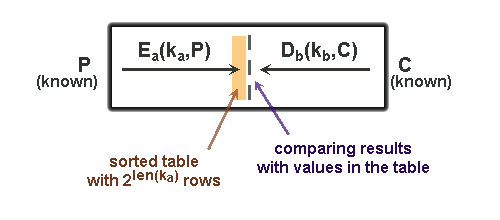
\includegraphics[width=.60\columnwidth]{attack_mitm_simple_eng}} \quad
\caption[Meet-In-The-Middle]{Darstellung einer Meet-In-The-Middle Attacke\footnotemark}
\label{fig:Pad0}
\end{figure}
\footnotetext{\cite{19}}
$\newline$
Wir brauchen dabei einen Klartext P und den dazugehörigen verschlüsselten Text C. Wir haben nun also: $$ P \rightarrow f(P,k_1) \rightarrow f(f(P,k_1), k_2) \rightarrow C $$
Der Trick ist nun den Zustand $ f(P,k_1)$ zu erreichen. Dabei wird zuerst ganz klassisch mit Brute-Force der Klartext P mit allen möglichen Schlüsseln ($2^{56} $ Bit) verschlüsselt und die Resultate gespeichert. Danach macht man das gleiche mit C und der Entschlüsselungsfunktion.

Es gilt also: $ P \rightarrow f(P,k_1) = d(C,k_2) \leftarrow C $

 Man vergleicht immer mit dem Resultat der Verschlüsselung von P. Es kann dabei mehrere Paare geben die zusammen passen, aber endlich viele. Diese kann man dann ausprobieren ob sie auch bei anderen verschlüsselten Texten funktionieren um so die richtigen 2 Schlüssel herauszufinden. \cite{19}

Größter limitierender Faktor war damals noch der hohe Speicherplatzverbrauch. Man brauchte die Kapazität die gesamten Intermediate Texte zu speichern. Das ist heutzutage kein Hindernis mehr. \cite{20}
$\newline$
Wenn man das Verfahren in 2 oder mehr einfachere Verfahren aufteilen kann, so ist es möglich eine sogeannte "'mehrdimensionale MitM Attacke"' durchzuführen. Dies  ist vor allem bei Blockchiffren ein Problem, die auf kleinen Datenblöcken mit sehr großen Schlüsseln agieren. Die Schlüssel werden hierbei effektiv aufgeteilt. 

$\newline$
\begin{figure}[h]
\centering
{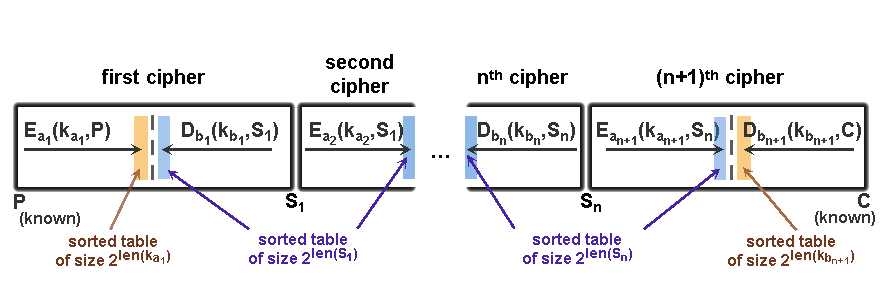
\includegraphics[width=.95\columnwidth]{attack_mitm_nd_eng}} \quad
\caption[mehrdimensionale MitM]{Darstellung einer mehrdimenionalen MitM Attacke\footnotemark}
\label{fig:Pad2}
\end{figure}
\footnotetext{\cite{19}
$\newline$

Schlussendlich bekommt man trotz der 2 verwendeten Schlüssel bei 2DES nicht eine resultierende Schlüssellänge von $2^{112} $ Bit, statdessen braucht man mit Brute-Force nur doppelt so lange um die Nachricht zu entschlüsseln, sollte man im Besitz eines Klartext- verschlüsselter Text Paares sein. Das enspricht $2^{57}$ Bit. Damit war 2DES nicht zukunftstauglich und wurde nicht in Betracht gezogen als Alternative für DES. \cite{18} 



\subsection{triple-DES}
3DES wurde im Standart X9.52 festgehalten und wurde zur neuen empfohlenen Verschlüsselungsmethode in der FIPS, der Federal Information Processing Standard. Dieser regelt die Standards, die Firmen erfüllen müssen um Verträge mit der US-Regierung zu schließen. Dies trug maßgeblich zu Verbreitung des 3DES in viele mit der Regierung zusammenhängenden Wirtschaftszweige bei. Zugleich wurde Single-DES oder DES nur noch für wenige, speziell zugelassene "'legacy systems"' erlaubt. Das sind Systeme die zu alt und groß waren, und die eher intern genutzt wurden. $\newline$
Zudem wurde die langsame Umstellung auf AES empfohlen, da dieser auch von der NSA speziell authorisiert war. Zunächst wollte man aber die hardwarebasierten DES-Systeme weiter nutzen, deswegen war 3DES ein logischer Schritt. \cite{21}
3DES basiert auf dem DES Algorithmus. Um etwas mit 3DES zu verschlüsseln nimmt man 2 DES Schlüssel mit jeweils 56 Bit und wendet sie wie folgt an: 
\begin{itemize}
\item Verschlüssele den Klartext mit dem ersten Schlüssel
\item Entschlüssle die Nachricht mit dem zweiten Schlüssel
\item Verschlüssle die Nachricht nochmal mit dem ersten Schlüssel
\end{itemize}
Diese besondere Anrt der Anwendug der 2 Schlüssel bedeutet eine Verlängerung des insgesamten Schlüssel auf 112 Bit. Dadurch ist er sehr viel schwerer mit Brute-Force zu knacken. \cite{6} 
Es hat keinerlei Auswirkungen auf die Sicherheit des Verfahrens ob man in Schritt 2 und 3 ver-oder entschlüsselt. Aber in der oben genannten Reihenfolge ist es üblich. Man kann nur nicht immer den gleichen Schlüssel benutzen. \cite{22}

Ein Nachteil von 3DES im Gegensatz zu anderen Verschlüsselungsverfahren ist seine Performanz. Da auf Hardwareverschlüsselung optimiert, ist die dreimalige Anwendung des DES-Algorithmus in Software form deutlich langsamer als von vergleichbaren Algorithmen mit ähnlich hoher Sicherheit. Deswegen ist 3DES im Privatgebrauch auch kaum verbreitet. Hier hat sich vor allem AES durchgesetzt wegen seiner sehr reduzierten Codebasis. \cite{23}

  


































%----------------------------------------------------------------------------------------
%	BIBLIOGRAPHY
%----------------------------------------------------------------------------------------

\renewcommand{\refname}{\spacedlowsmallcaps{References}} % For modifying the bibliography heading

\bibliography{literatur}
\bibliographystyle{ieeetr}

%----------------------------------------------------------------------------------------

\end{document}
